\documentclass[10pt]{article}
\usepackage[margin=0.9in]{geometry}
\usepackage{amsmath,amssymb,amsthm}
\usepackage{booktabs}
\usepackage{graphicx}
\usepackage{enumitem}
\usepackage{xcolor}
\usepackage[section]{placeins}
\usepackage[colorlinks=true,linkcolor=blue!50!black,citecolor=blue!50!black,urlcolor=blue!50!black]{hyperref}
\setlist{nosep,leftmargin=1.4em}
\setlength{\parskip}{3pt}
\setlength{\parindent}{0pt}

\newcommand{\Rp}{\mathsf{R}}
\newcommand{\Op}{\mathsf{O}}
\newcommand{\bx}{\mathbf x}
\newcommand{\by}{\mathbf y}
\newcommand{\bG}{\mathbf G}
\newcommand{\bA}{\mathbf A}
\newcommand{\bb}{\mathbf b}
\newcommand{\bM}{\mathbf M}
\newcommand{\bbeta}{\boldsymbol\beta}
\newcommand{\btheta}{\boldsymbol\theta}
\newcommand{\unverified}[1]{\textcolor{orange!70!black}{[unverified: #1]}}
\newtheorem{proposition}{Proposition}
\renewcommand{\theproposition}{A\arabic{proposition}}
\newtheorem{remark}{Remark}

\newcommand{\CommJointSevenBig}{18}
\newcommand{\CommPerSeven}{0.9}
\newcommand{\CommPerSevenBig}{2.8}
\newcommand{\CostBase}{85}
\newcommand{\CostJointSeven}{15.8}
\newcommand{\CostJointSevenBig}{3.2}
\newcommand{\CostPerSeven}{7.5}
\newcommand{\CostPerSevenBig}{19}
\newcommand{\EXIrmse}{0.025}
\newcommand{\EXprec}{99.99\%}
\newcommand{\EXrec}{78.3\%}
\newcommand{\EXrecMNAR}{62.8\%}
\newcommand{\FBexrec}{42.6\%}
\newcommand{\FBmkrec}{79.6\%}
\newcommand{\FormulaRfive}{0.950}
\newcommand{\FormulaRone}{0.992}
\newcommand{\FormulaRten}{0.897}
\newcommand{\LSHIrmse}{0.044}
\newcommand{\LSHcovR}{0.419}
\newcommand{\LSHcovRfour}{0.001}
\newcommand{\LSHmultiCand}{1{,}839{,}977}
\newcommand{\LSHmultiN}{3{,}000{,}000}
\newcommand{\LSHnoncohort}{11{,}777}
\newcommand{\LSHprec}{77.9\%}
\newcommand{\LSHratioR}{0.766}
\newcommand{\LSHrec}{72.4\%}
\newcommand{\MKIrmse}{0.021}
\newcommand{\MKfalse}{0.69\%}
\newcommand{\MKnoncohort}{360}
\newcommand{\MKprec}{99.31\%}
\newcommand{\MKrec}{97.0\%}
\newcommand{\MKrecMNAR}{88.7\%}
\newcommand{\MKtwoprec}{99.97\%}
\newcommand{\MKtworec}{87.7\%}
\newcommand{\NoffIfour}{7{,}286}
\newcommand{\NoffIone}{27{,}046}
\newcommand{\PerfIrmse}{0.020}
\newcommand{\SwCovRfourFive}{0.535}
\newcommand{\SwCovRfourTen}{0.302}
\newcommand{\SwCovRfourTwo}{0.840}
\newcommand{\SwCovRfourZero}{0.948}
\newcommand{\SwCovRoneFive}{0.865}
\newcommand{\SwCovRoneTen}{0.703}
\newcommand{\SwCovRoneTwenty}{0.407}
\newcommand{\SwCovRoneZero}{0.953}
\newcommand{\SwMNARcovOfour}{0.298}
\newcommand{\SwMNARcovRfour}{0.205}
\newcommand{\SwMNARratio}{0.839}
\newcommand{\SwMNARratioO}{0.844}


\title{\textbf{Probabilistic record linkage through the protocol's OPRF-PSI:\\ is it a valid idea?}}
\author{Research note on protocol v3.1 (\texttt{paper/main.tex}, \texttt{docs/protocol\_v31.tex})}
\date{2026-10-27}

\begin{document}
\maketitle

\begin{abstract}
\noindent Protocol v3.1 links $\Rp$'s cohort to $\Op$'s register by labeled PSI on 2HashDH OPRF values of a clean shared identifier. We ask whether the same machinery can link on noisy quasi-identifiers (name, date of birth, postcode), accepting false and missed matches, against honest-but-curious parties. Exact-match PSI can only test equality, so approximate matching has to be reduced to equality of \emph{derived keys}. We analyse three reductions (several error-tolerant keys with an OR rule, LSH keys, and per-field tokens scored after the PSI), what each changes in the protocol (item uniqueness, many-to-many candidates, cost, leakage, DP sensitivity), and the statistical consequences for the regression, and we test them on synthetic records with realistic corruption and on FEBRL4. \textbf{Verdict: partially valid.} Multiple deterministic keys with an OR rule, a uniqueness filter at $\Op$, a 1:1 resolution at $\Rp$ and per-type PSI instances fit the protocol with small changes and work well. On a $10^6$-row register they find \MKrec\ of the true pairs at precision \MKprec, against \EXrec\ for exact matching on the clean quasi-identifiers. The DP guarantee is unchanged, provided the linkage uses no DP-protected variable and the alignment is injective on $\Op$'s rows. What does not carry over is the disclosure guarantee G4: $\Rp$ learns key-level match patterns, including the positions of non-cohort people who share a key. Linkage error also biases the coefficients of $\Rp$'s own features, by the factor $1-\pi$ (the false-match rate) to first order, and the bias-aware interval does not cover this bias once $\pi$ is a few percent at large $n$. LSH keys are not viable at register scale in this design. Private field-level scoring needs circuit-PSI or another protocol for computing on the intersection, not labeled PSI.
\end{abstract}

\tableofcontents

% ======================================================================
\section{What the alignment computes today}
\label{sec:now}

\paragraph{The Link phase (paper, Section~6 and Appendix~C; specification, Algorithm~2).}
$\Op$ pads its scope register to the public size $\bar n_O$, draws a fresh OPRF key $k$ and a uniformly random shuffle $\tau$ every run, and inserts the item $F_k(\mathrm{id}_j)$ with label $\tau(j)$, masked by a key derived from $F'_k(\mathrm{id}_j)$. Items are 64 bits, two field elements (``felts'') modulo $t\approx2^{32}$. They are hashed into $2^{14}$ bins with $h=3$ functions and split into partitions of degree $D=64$. $\Rp$ pads its identifiers to $n_R^{\max}$ and obtains $F_k$ on them through the blinded 2HashDH exchange (RFC~9497~\cite{rfc9497,jarecki2014round}): $\Op$ sees only uniform group elements, and $\Rp$ never learns $k$. $\Rp$ cuckoo-hashes its items, at most one per bin, with an augmenting-path fallback, and sends BFV-encrypted windowed powers. $\Op$ evaluates the masked membership and label polynomials and floods the replies (\textsc{SanitizeBFV}). $\Rp$ declares a match only if all felts are zero and the label felts agree. It aborts if one identifier gets two positions, or if two identifiers get the same position (\texttt{psi.receiver\_decode}, \texttt{psi.check\_injective}).

\paragraph{Who learns what.} $\Op$ learns nothing beyond $(n_R^{\max},\bar n_O)$ (G1, G2), up to the cuckoo and false-match slack. $\Rp$ learns $I$, the cohort members in scope, and the positions $\pi|_I$ (G4). G4 is proved in the random-oracle model under CDH (proofs, Part~A, Lemma~7.2 and Theorem~7.3). The simulator gets $(I,\pi|_I)$ and the public sizes; items and labels of rows outside $I$ are pseudorandom to $\Rp$. Intersection size: $\Rp$ learns $n=|I|$, and $\Op$ does not.

\paragraph{Key holder and dictionary attacks.} The OPRF key is $\Op$'s, and $\Op$ is also the party that holds every item in the clear. $\Rp$ cannot evaluate $F_k$ offline, so it cannot run a dictionary attack against $\Op$'s items. Each membership test costs an online OPRF call, and the calls are capped by the padded count $n_R^{\max}$ per run and by a cross-session quota. $\Op$ cannot attack $\Rp$'s identifiers: the blinded elements are uniform and the PSI query is under $\Rp$'s own BFV key.

\paragraph{DP.} The adjacency (paper, Definition~1) holds the identifiers, $\Phi$ and the cohort fixed and changes one row's $(\bx_O,y)$. Hence the linkage, and the whole PSI transcript, is the same on neighbouring datasets. Theorem~1 states that PSI security is not needed for G3. The replace-one sensitivity $\Delta$ (Proposition~1) assumes that each of $\Op$'s positions carries at most one row of $\Rp$ ($b_t\in\{0,1\}$).

% ======================================================================
\section{Mechanisms for approximate matching on top of exact PSI}
\label{sec:mech}

The PSI tests equality of byte strings and nothing else. Every approximate scheme built on it must therefore map a record to a set of \emph{keys}, so that similar records share at least one key with useful probability and dissimilar records rarely do. Otherwise the equality primitive has to be replaced. Every scheme below feeds keys to the OPRF exactly as the identifier is fed today. Keys are domain-separated by a type index, so a key of type $\kappa$ can only meet a key of type $\kappa$. All parameters (key definitions, the nickname table, $K$) are public and agreed in Setup.

\subsection{(a) Several error-tolerant keys with an OR rule}
Each record yields $K$ keys. A pair becomes a \emph{candidate} if at least one key agrees, and the set of agreeing key types is its \emph{pattern}. Our multikey scheme ($K=7$, \texttt{keys.py}) uses:
\begin{center}\small
\begin{tabular}{@{}lll@{}}
\toprule
key & content & tolerates \\
\midrule
$k_1$ & canonical first name $|$ surname $|$ DOB & nicknames (public nickname table)\\
$k_2$ & NYSIIS(first) $|$ NYSIIS(surname) $|$ DOB & spelling variants, many typos\\
$k_3$ & Soundex(surname) $|$ initial $|$ sex $|$ year $|$ \{day, month\} unordered & day--month swap, first-name typos\\
$k_4$ & first $|$ surname $|$ postcode & any DOB error\\
$k_5$ & Metaphone(first) $|$ Metaphone(surname) $|$ year $|$ month & day typo\\
$k_6$ & first $|$ sex $|$ DOB $|$ postcode & surname change\\
$k_7$ & surname $|$ sex $|$ DOB $|$ postcode & first-name error or missing\\
\bottomrule
\end{tabular}
\end{center}
This is the PSI version of deterministic, rule-based ``match-key'' linkage as used by statistical agencies. One example is the hierarchical match keys used to link census and administrative data at the UK ONS \unverified{we did not check the ONS key definitions or their published error rates}. Each key must keep enough entropy to be nearly unique in a register of $\bar n_O$ rows, which is why every key combines at least three fields.

\subsection{(b) LSH keys}
Locality-sensitive hashing turns a similarity into a collision probability. MinHash~\cite{broder1997resemblance} over character $q$-grams with $b$ bands of $r$ hashes makes two strings of $q$-gram Jaccard similarity $J$ share at least one band key with probability $1-(1-J^r)^b$. SimHash~\cite{charikar2002similarity} does the same for cosine similarity, and Hamming-LSH, which samples bit positions, does it for Bloom-filter encodings of $q$-grams (cryptographic long-term keys, CLKs) in the style of Schnell et al.~\cite{schnell2009privacy}. A Bloom filter is \emph{not} itself an equality token. Using it here would mean Hamming-LSH bands of the filter, which are again keys. Uzun et al.~\cite{uzun2021fuzzy} build fuzzy labeled PSI for biometric search exactly this way: LSH subsamples become items of a labeled PSI, and a match needs $t$ out of $T$ agreements. Our LSH scheme uses 24 MinHash functions in 8 bands of 3 over the bigrams of ``first surname''. Each band key is joined with the birth year to add entropy, giving $K=8$.

LSH has a structural problem at register scale, which the experiments confirm (Section~\ref{sec:exp}). A band key is low-entropy \emph{by design}, because it must collide for similar strings. It is therefore shared by many register rows, so either it is removed by $\Op$'s uniqueness filter, which destroys recall, or it returns many positions, which multiplies the candidates and the leakage.

\subsection{(c) Per-field tokens and Fellegi--Sunter scoring after the PSI}
Fellegi--Sunter (FS) linkage~\cite{fellegi1969theory} scores a pair by its field agreement vector $\gamma$, with weights $\log_2(m_f/u_f)$ for agreement and $\log_2((1-m_f)/(1-u_f))$ for disagreement. The weights are usually fitted by EM~\cite{winkler1988using}. It cannot be run by PSI on fields alone: a field such as sex or birth year matches a large part of the register. It needs blocking first. Three realisations:
\begin{enumerate}[label=(c\arabic*)]
\item \emph{Blocking PSI with field tokens in the label.} Blocking keys (e.g.\ the multikey set) form the PSI items. The label carries, besides $\tau(j)$, one OPRF-derived token per field of $\Op$'s row, which $\Rp$ compares with its own tokens. $\Rp$ then learns the full agreement vector $\gamma$ of every candidate pair. That is the classic leakage of PPRL with encoded fields. The OPRF prevents offline guessing of the field values, but equality patterns over many pairs are exactly what frequency and pattern-mining attacks exploit~\cite{kuzu2011constraint,niedermeyer2014cryptanalysis,vidanage2019efficient}.
\item \emph{Circuit-PSI with payloads, then secure scoring.} Circuit-PSI~\cite{pinkas2019efficient,rindal2021vole} leaves the membership bit and the payloads (field tokens) \emph{secret-shared}. A garbled circuit or an HE computation then computes $\gamma$, the FS score and the threshold, and reveals only the decision and, for accepted pairs, the position. The 1:1 resolution of conflicting candidates must also run in MPC, which needs oblivious sorting or an oblivious assignment. That is a substantial addition. It would also hide $I$ from $\Rp$, which moves the design to the membership-hiding variant (paper, Remark~13): $\bA$ is no longer exact, the aggregation moves off CKKS, and the adjacency must cover match status.
\item \emph{Fuzzy PSI primitives.} Protocols that intersect under a distance replace equality by ``within distance $\delta$''. They include Freedman--Nissim--Pinkas fuzzy matching~\cite{freedman2004efficient}, found flawed and repaired by Chmielewski and Hoepman~\cite{chmielewski2008fuzzy}; Indyk--Woodruff~\cite{indyk2006polylogarithmic}; structure-aware PSI for Hamming and $\ell_\infty$ balls~\cite{garimella2022structure}; distance-aware PSI~\cite{chakraborti2023distance}; and fuzzy PSI with large hyperballs~\cite{vanbaarsen2024fuzzy}. They handle numeric vectors or Hamming distance on fixed-length strings. As far as we know, none handles multi-field string comparison with frequency-dependent FS weights, labeled output, and the 1:1 resolution this protocol needs. The fuzzy PSI paper by ``Garimella et al.'' named in the request is, we believe, \cite{garimella2022structure} \unverified{a different Garimella et al.\ fuzzy-PSI paper may have been meant}.
\end{enumerate}
Secure PPRL by MPC has a separate literature: hybrid blocking plus secure computation~\cite{inan2008hybrid}, and DP blocking composed with secure matching~\cite{he2017composing}. The PPRL taxonomy and survey literature~\cite{vatsalan2013taxonomy,christen2020linking} cover Bloom-filter linkage and its attacks in depth. \unverified{We could not identify the ``Lindell secure PPRL'' reference in the request with confidence and do not cite one.}

\subsection{Resolution at $\Rp$}
\label{sec:resolve}
After the PSI, $\Rp$ holds candidate pairs (record $i$, position $t$) with their key patterns. It weights them by FS, with $u_\kappa$ estimated as the random-pair agreement rate of key $\kappa$ within $\Rp$'s \emph{own} file (no data from $\Op$) and $m_\kappa$ by EM with $u$ fixed. It then accepts pairs in decreasing weight order, at most one per record and one per position. A record or position whose two best candidates tie is dropped as ambiguous. An optional rule requires at least $k_{\min}$ agreeing keys. A fully unsupervised EM fit of $(m,u)$ on the candidate set behaved badly in our tests. The candidates are almost all true matches, so the ``non-match'' class absorbed true matches with unusual patterns, and recall fell from 0.97 to 0.83 at no gain in precision. That is why $u$ is fixed from random pairs. All of this is post-processing of $\Rp$'s PSI output.

% ======================================================================
\section{What breaks or changes in this protocol}
\label{sec:changes}

\subsection{Unique items and the abort rule}
The labeled PSI holds one label per item. Identical items from two of $\Op$'s rows land in different partitions of the same bin (\texttt{psi.\_greedy\_bin}). $\Rp$ then sees one item matched at two positions, which the paper's recovery rule treats as an abort, and the implementation raises an error once the duplicates exhaust a bin's partitions. With quasi-identifier keys, duplicates in $\Op$'s register are normal: twins, namesakes in one household, common names. $\Op$ must therefore make every key value unique before insertion. There are two policies:
\begin{itemize}
\item \textbf{uniqueness filter} (\texttt{unique}): $\Op$ deletes every key value held by more than one of its rows and puts a fresh random dummy item in its place, so that each key type still has exactly $\bar n_O$ items and the sizes stay public. This filter is what makes deterministic keys safe at scale. It removes exactly the keys that would produce ambiguous candidates, and it adds no leakage: a non-unique value looks the same to $\Rp$ as an absent one.
\item \textbf{multi-label} (\texttt{multi}): the label carries every position with that value, padded to a public cap $c_{\max}$. This needs a label of $c_{\max}$ positions, so $c_{\max}$ times the label polynomials and replies. It reveals each matched value's multiplicity up to $c_{\max}$, and it is \emph{not} supported by the current implementation. We simulate it as an ablation.
\end{itemize}
On $\Rp$'s side, $\Rp$ queries each distinct key value once and fans the result out to the records that share it. The injectivity check must change. Two key types of one record legitimately return the same position, and two records may return the same position. The second case goes to the resolution step instead of an abort. A genuine PSI false match (probability $\le p_{\mathrm{pass}}\approx2^{-67}$ per run at the evaluation sizes, times $K$) could then pass silently instead of aborting. That is a correctness event already covered by $\delta_{\mathrm{psi}}$. Padding becomes $K$ keys per padded record, with random dummies for missing fields, so $\Op$ still sees exactly $K n_R^{\max}$ blinded elements and G1--G2 keep their form with $K$ public.

\subsection{Many-to-many candidates and the 1:1 alignment}
The upload writes \emph{one} row of $\Rp$ per position $t$, in $\tau$-order, with the selection bit $b_t$. A position cannot carry two of $\Rp$'s rows without duplicating the upload vectors, so the alignment must be injective on $\Op$'s positions. That is also what keeps the sensitivity unchanged (Proposition~\ref{prop:sens}). An $\Rp$ record could legally sit at two positions (one-to-many on $\Rp$'s side) without any effect on DP, but every extra position is a likely false match. The greedy 1:1 resolution of Section~\ref{sec:resolve} gives an injective alignment without further interaction or leakage. The alternative is to drop every ambiguous record and position (``unambiguous'' rule, \texttt{linkage.resolve}). It is safer but loses recall wherever candidates conflict.

\subsection{Cost}
With $K$ keys, $\Op$ evaluates its OPRF on $K\bar n_O$ inputs and $\Rp$ sends $K n_R^{\max}$ blinded elements and PSI items. The CKKS part is unchanged, because it runs over the $\bar n_O$ positions whatever the linkage. How the Link phase scales depends on the layout (\texttt{cost.py}, from the repo's refreshed cost model \texttt{implementation/bench/cost\_model.py}, Table~\ref{tab:cost}):
\begin{itemize}
\item \textbf{one joint PSI} over all keys: $\Op$'s evaluation and the replies cost (cuckoo tables) $\times$ (partitions per bin), and both grow with $K$. The cost therefore grows like $K^2$, and faster at large $n_R^{\max}$, where the $\delta_{\mathrm{psi}}$ bound on cuckoo failure forces more, emptier tables;
\item \textbf{$K$ PSI instances, one per key type}, each of today's size: the output to $\Rp$ is identical, because keys are domain-separated, and every Link phase costs $K$ times today's. This is the layout to use.
\end{itemize}
\begin{table}[t]\centering\small
\caption{Modelled cost of one run with $K$ keys per record at $\bar n_O=1{,}007{,}616$ (refreshed cost model; 4 threads per
party; $\Op$'s wall time in minutes, total traffic in GB). Joint: one PSI over all keys (tables/partitions per bin
shown); per type: $K$ PSI instances of today's size. $K=1$ is today's protocol ($85$\,s modelled, $91$\,s measured at
$n_R^{\max}=20{,}000$). Beyond $K=1$ these are model extrapolations, not measurements.}\label{tab:cost}
\begin{tabular}{@{}rrrrrrr@{}}\toprule
 & & \multicolumn{3}{c}{joint PSI} & \multicolumn{2}{c}{per-type PSI}\\\cmidrule(lr){3-5}\cmidrule(lr){6-7}
$n_R^{\max}$ & $K$ & $\Op$ (min) & traffic (GB) & tables / $\alpha$ & $\Op$ (min) & traffic (GB)\\\midrule
20{,}000 & 1 & 1.4 & 0.46 & 2 / 5 & 1.4 & 0.46 \\
20{,}000 & 2 & 2.9 & 0.56 & 4 / 9 & 2.4 & 0.53 \\
20{,}000 & 4 & 6.9 & 0.84 & 8 / 16 & 4.5 & 0.67 \\
20{,}000 & 7 & 15.8 & 1.45 & 14 / 26 & 7.5 & 0.88 \\
20{,}000 & 8 & 19.3 & 1.70 & 16 / 29 & 8.5 & 0.94 \\
20{,}000 & 12 & 40.8 & 3.22 & 27 / 41 & 12.5 & 1.22 \\
\addlinespace
100{,}000 & 1 & 3.1 & 0.74 & 10 / 5 & 3.1 & 0.74 \\
100{,}000 & 2 & 8.1 & 1.24 & 20 / 9 & 5.8 & 1.08 \\
100{,}000 & 4 & 42.3 & 4.57 & 75 / 16 & 11.3 & 1.77 \\
100{,}000 & 7 & 190.8 & 17.58 & 229 / 26 & 19.4 & 2.80 \\
100{,}000 & 8 & 274.1 & 24.59 & 299 / 29 & 22.1 & 3.14 \\
100{,}000 & 12 & 843.4 & 70.52 & 672 / 41 & 33.0 & 4.52 \\
\bottomrule\end{tabular}\end{table}


\subsection{Leakage: G4 must be restated}
\label{sec:leak}
Theorem~7.3's simulator needs only $\Rp$'s output and the public sizes, and its proof never uses the fact that the items are identifiers. It uses that $\Rp$ queries a fixed padded list and that $\Op$'s items outside that list are pseudorandom (Lemma~7.2). With keys, $\Rp$'s output becomes the \emph{key-level match function}
\[
  \mathcal L_K=\bigl\{(i,\kappa,\tau(j)) : \mathrm{key}_\kappa(r_i)=\mathrm{key}_\kappa(o_j)\ \text{and that value is unique among }\Op\text{'s rows}\bigr\},
\]
and the same argument proves G4 with $(I,\pi|_I)$ replaced by $\mathcal L_K$. One condition is that $\Op$ refills filtered and missing keys with random dummies, so that the number of items per type stays public. G4 therefore \emph{holds in form but discloses more}. What $\Rp$ learns beyond exact linkage:
\begin{enumerate}
\item \textbf{agreement patterns} for its cohort members: which keys of $\Op$'s copy agree with its own (e.g.\ ``$\Op$ has a different surname or postcode for this person'');
\item \textbf{positions of non-cohort people}: a key shared with somebody else in the register returns that person's row, and $\Rp$ learns that a person with that key value (a phonetic name, a DOB, a postcode) is in $\Op$'s scope. Table~\ref{tab:linkage} counts these rows: \MKnoncohort\ for $50{,}000$ cohort records with the multikey scheme on a $10^6$-row register, \LSHnoncohort\ with LSH keys;
\item \textbf{cross-key profiles}: within a run, every key of row $j$ carries the same label $\tau(j)$. Hits from several keys, or from several of $\Rp$'s records, on one position tell $\Rp$ that a single row of $\Op$ has all those key values. Hiding this join would need per-type secret positions, which the upload cannot use, or secret-shared output (circuit-PSI);
\item with the multi-label ablation, \textbf{multiplicities} of matched key values.
\end{enumerate}
With a fresh key and $\tau$ every run, none of this can be linked across runs. $\Op$'s view does not change.

\paragraph{Dictionary and frequency attacks.} The OPRF still blocks offline guessing by $\Rp$. $\Op$, the key holder, cannot attack $\Rp$, because it never sees $\Rp$'s values, OPRF outputs or PSI items. This is a real advantage over Bloom-filter PPRL, where a linkage unit holds encodings of both files and can run frequency and pattern-mining attacks~\cite{kuzu2011constraint,niedermeyer2014cryptanalysis,christen2018precise}. Low-entropy keys change the picture. Each of $\Rp$'s queries becomes a membership test on a whole equivalence class, so even an honest $\Rp$ learns more. The $K n_R^{\max}$ query budget of a run is also large next to small key spaces. For example, $k_3$ ranges over about $5{,}000$ (Soundex) $\times26\times2\times70\times78\approx5\times10^{10}$ values, but an LSH band${}\times{}$year key is shared by many people by design. A $\Rp$ that deviated from the protocol (outside the honest-but-curious model) could spend its budget mapping the register's frequency structure. Against honest-but-curious parties the relevant quantity is the honest leakage $\mathcal L_K$, and key entropy controls it.

\subsection{DP sensitivity}
\begin{proposition}[Sensitivity with approximate linkage]\label{prop:sens}
Let the alignment (the candidates and the resolution) be a function of the quasi-identifiers, $\Rp$'s data and public parameters only, and let the quasi-identifiers be held fixed by the adjacency, as the identifiers are in Definition~1.
\begin{enumerate}[label=(\roman*)]
\item If every position of $\Op$ carries at most one row of $\Rp$, the replace-one sensitivity is exactly $\Delta$ of the paper's Proposition~1, and the paper's Theorem~1 and the ledger apply unchanged. $\Rp$-side one-to-many does not matter.
\item If a position may carry up to $m$ rows of $\Rp$ (no resolution, replicated uploads), the released statistic is a sum over pairs, and replacing one row of $\Op$ changes up to $m$ pairs. Then $\Delta_m\le m\Delta$, with equality when the $m$ rows of $\Rp$ are equal. The noise must scale with a public cap $m_{\max}$: $\sigma\times m_{\max}$, or $\rho\times m_{\max}^2$ at fixed $\sigma$.
\item If a matching field is also a protected variable, or a function of one (age from DOB, region from postcode, sex as a covariate in $\bx_O$), the alignment depends on $(\bx_O,y)$. Neighbouring datasets then differ in match status as well, the PSI transcript is no longer independent of the protected data, and $\Rp$'s key patterns reveal those fields of matched rows outside DP. Such variables must either be excluded from the keys or be treated as disclosed for linked records.
\end{enumerate}
\end{proposition}
\begin{proof}
(i) The PSI output, the uniqueness filter and the resolution are fixed under $\sim$, so $\bb$ and $\dot{\mathbf X}_R$ are fixed. Replacing row $j$ changes only the terms of the single pair at $\tau(j)$, which is the setting of the paper's Proposition~1. (ii) Each statistic is $\sum_t\sum_{i\to t}g(\dot\bx_i,\bx_t,y_t)$. Replacing row $t$ changes $\sum_{i\to t}[g(\dot\bx_i,\bx,y)-g(\dot\bx_i,\bx',y')]$, whose norm is at most $m\Delta$ by the triangle inequality. With equal $\dot\bx_i$ the sum is $m$ times one change, which attains $m\Delta$ at the maximiser of the paper's Proposition~1. (iii) The alignment is then a function of $(\bx_O,y)$, so the premise of the paper's Proposition~1 (fixed $\bb$) fails, and so does Theorem~1's remark that the PSI transcript does not depend on $(\bx_O,y)$.
\end{proof}
The candidates \emph{before} resolution do not matter for DP. They are a function of quasi-identifiers only, and only the final alignment enters the statistics. Linkage error is therefore a statistical problem here, not a privacy one, as long as (i) and (iii) hold.

% ======================================================================
\section{Statistical consequences for the regression}
\label{sec:stats}

\paragraph{False matches as contamination.} Let a fraction $\pi$ of the linked pairs be false. Model a false match as pairing $\Rp$'s $\dot\bx_R$ with the $(\bx_O,y)$ of a person drawn independently from $\Op$'s scope, the exchangeable linkage-error model behind Neter et al.~\cite{neter1965effect}, Scheuren and Winkler~\cite{scheuren1993regression} and Lahiri and Larsen~\cite{lahiri2005regression}. In this protocol $y$ is $\Op$'s and travels with $\bx_O$. A false match therefore keeps the $\bx_O$--$y$ relation intact and breaks only the link between $\Rp$'s block and $\Op$'s. With $\bM=E[\mathbf z\mathbf z^\top]$ and $\mathbf m=E[\mathbf z y]$ over true pairs, and $\bM_{\perp},\mathbf m_\perp$ the same under independent pairing (whose $\Rp$--$\Op$ blocks are products of means), least squares converges to
\begin{equation}\label{eq:contam}
  \btheta^*(\pi)=\bigl((1-\pi)\bM+\pi\bM_\perp\bigr)^{-1}\bigl((1-\pi)\mathbf m+\pi\mathbf m_\perp\bigr).
\end{equation}
For centred features with uncorrelated blocks ($\Sigma_{RO}=0$), \eqref{eq:contam} reduces to
\[
  \btheta^*_R=(1-\pi)\bbeta_R,\qquad \btheta^*_O=\bbeta_O .
\]
$\Rp$'s coefficients are attenuated by exactly the false-match rate, and $\Op$'s are unbiased. With correlated blocks, part of $\Rp$'s lost signal moves to the correlated features of $\Op$ (omitted-variable shift). In the paper's synthetic population (Toeplitz correlation $0.3$), \eqref{eq:contam} gives an average ratio $\theta^*_R/\beta_R$ of \FormulaRone, \FormulaRfive\ and \FormulaRten\ at $\pi=0.01,0.05,0.10$, while $\Op$'s ratios stay within $2\%$ of 1. This is the worst place for the bias to fall. The paper's scope is whether \emph{$\Rp$'s} cohort covariates predict $\Op$'s outcome, and $\Rp$'s coefficients are exactly what contamination shrinks. Contamination that is not exchangeable, e.g.\ false matches within a household or birth cohort that share covariates, attenuates less but in a way that depends on the data. Corrections that use match probabilities exist~\cite{lahiri2005regression,chambers2009regression}, and Lin, Paquette and Kolaczyk~\cite{lin2024differentially} combine linkage error with central DP for linear regression.

\paragraph{Missed matches.} Missing at random lowers $n$ without bias. The DP noise does not shrink with $n$, so the relative noise grows. Below $n_{\mathrm{off}}$ (\NoffIone\ matched records at $\varepsilon=1$ and \NoffIfour\ at $\varepsilon=4$ in setting~I for this population) the stage-1 rule turns the ridge on, which adds a bias that the bias-aware interval does cover. Misses that depend on the outcome select on $y$ and bias every coefficient towards zero. Misses that depend on covariates alone do not bias a correctly specified linear model.

\paragraph{Intervals.} The Wald interval targets $\btheta_\lambda=(\bG+\lambda\Psi)^{-1}\mathbf c$ computed on \emph{the linked rows}, so it keeps its coverage under any linkage error. But that estimand is the contaminated one. The bias-aware interval for $\bbeta$ covers the ridge bias and the mechanism noise, not the linkage bias $\pi\bbeta_R$. It fails once $\pi|\beta_{R,j}|$ is comparable to its half-width, which shrinks with $n$ and $\varepsilon$. More data and more budget therefore make the problem \emph{worse} in relative terms (Table~\ref{tab:sweep}).

\paragraph{A moment correction, and why it is not enough.} Under the exchangeable model $E[\tilde\bG_{RO}]=(1-\pi)\bG_{RO}+\pi n\,\bar{\dot\bx}_R\mu_O^\top$ and $E[\tilde{\mathbf c}_R]=(1-\pi)\mathbf c_R+\pi n\,\bar{\dot\bx}_R\mu_y$. The $\Op$--$\Op$ blocks and $\mathbf c_O$ are unaffected. Given $\pi$ and the scope means $(\mu_O,\mu_y)$, $\Rp$ could undo the attenuation. The means are $\Op$ statistics and would need a (cheap) DP release. The hard part is $\pi$. $\Rp$ cannot audit links, because it never sees $\Op$'s data, so $\pi$ must come from the linkage model, and FS posteriors are known to be poorly calibrated~\cite{winkler1988using}. Our EM experience (Section~\ref{sec:resolve}) agrees. An interval that is valid under linkage error would also have to carry the uncertainty in $\pi$. We leave both open.

% ======================================================================
\section{Experiments}
\label{sec:exp}

\paragraph{Why a plaintext simulation is exact.} The OPRF is a PRF evaluated under one key on both sides, so two keys meet iff the strings are equal, up to the PSI's own correctness failures, which are bounded by $\delta_{\mathrm{psi}}+p_{\mathrm{pass}}$ and set to $\le2^{-40}$ by Setup. The labeled PSI returns, for each queried item, its label if $\Op$ inserted it. Its output on the keys is therefore exactly a dictionary lookup of $\Rp$'s keys in $\Op$'s key$\to$position map, which \texttt{linkage.psi\_output} computes. The shuffle $\tau$ is a relabelling that changes nothing downstream. The regression runs on the linked statistics $(\bG,\mathbf c,\by^\top\by)$ through the repo's own release and solve code. This is the same plaintext path as the paper's large-$n$ simulation (\texttt{experiments/large/sim\_large.py}), and the encrypted protocol reproduces it to about $10^{-10}$.

\paragraph{Data.} \texttt{generator.py} builds a population of people in households of 1--4 sharing a postcode and (85\%) a surname, with 1.5\% twins (same DOB and surname). First names follow a Zipf--Mandelbrot law over common English and French names plus a synthetic tail (top name about 4\%), and surnames the same over about $60{,}000$ types (top surname 0.6\%, top 100 cover 22\%). DOB spans 1935--2005, with sex and a postcode. Regression variables come from the paper's synthetic population ($d_R=4$, $d_O=6$, $R^2=0.5$, \texttt{std} preprocessing), independent of the quasi-identifiers. Each copy is corrupted independently, $\Rp$'s more than $\Op$'s. Per record, $\Rp$'s rates are: nickname or variant 8\%, first-name typo 3\%, surname typo 3\%, surname change for women 22+ 8\%, day--month swap 2\%, DOB digit typo 2\%, moved 15\%, and missing values 0.5--1\%. These rates are assumptions, not estimates for any register. Main world: $\Op$ scope $10^6$ rows; $\Rp$ cohort $50{,}000$, of whom $40{,}000$ are in scope. A second world (seed 2) makes every corruption rate twice as high for people whose outcome is below the median (\emph{MNAR}). FEBRL4~\cite{christen2008febrl} (5,000 records and 5,000 heavily corrupted duplicates) serves as an external check of the key schemes.

\subsection{Linkage quality and leakage}
\begin{table}[t]\centering\small
\caption{Linkage on the synthetic world ($\Op$: $10^6$ rows; $\Rp$: 50{,}000 records, 40{,}000 in scope). Precision and recall
of the accepted 1:1 links against the truth; candidate recall: true pairs among the PSI candidates (the ceiling of any
resolution); candidate pairs and non-cohort positions: what $\Rp$ learns from the PSI (Section~\ref{sec:leak}). Last two
columns: the MNAR world (corruption doubled for outcomes below the median). The FS rows score the candidates of the multi-label multikey blocking. $^\dagger$Not supported by the current PSI
(one label per item).}\label{tab:linkage}
\resizebox{\textwidth}{!}{\begin{tabular}{@{}lrrrrrrrr@{}}\toprule
scheme & $K$ & precision & recall & cand.\ recall & cand.\ pairs & non-cohort pos. & prec.\ MNAR & rec.\ MNAR\\\midrule
exact QIs ($K{=}1$) & 1 & 99.99\% & 78.3\% & 78.3\% & 31{,}305 & 2 & 99.99\% & 62.8\% \\
multikey, filter, $\ge1$ key & 7 & 99.31\% & 97.0\% & 97.0\% & 39{,}195 & 360 & 99.12\% & 88.7\% \\
multikey, filter, $\ge2$ keys & 7 & 99.97\% & 87.7\% & 97.0\% & 39{,}195 & 360 & 99.96\% & 76.0\% \\
multikey, multi-label$^\dagger$ & 7 & 99.31\% & 97.0\% & 97.1\% & 40{,}822 & 1{,}889 & 99.12\% & 88.7\% \\
LSH, filter, $\ge1$ band & 8 & 77.95\% & 72.4\% & 73.0\% & 41{,}607 & 11{,}777 & 72.09\% & 63.8\% \\
LSH, filter, $\ge2$ bands & 8 & 97.13\% & 51.1\% & 73.0\% & 41{,}607 & 11{,}777 & 96.21\% & 44.6\% \\
FS on field tokens (c1), $p\ge0.5$ & 9 & 99.33\% & 97.0\% & -- & 40{,}822 & 1{,}889 & 99.13\% & 88.8\% \\
FS on field tokens (c1), $p\ge0.999$ & 9 & 99.37\% & 97.0\% & -- & 40{,}822 & 1{,}889 & 99.17\% & 88.8\% \\
\bottomrule\end{tabular}}\end{table}

\begin{table}[t]\centering\small
\caption{FEBRL4 (5{,}000 originals as $\Op$, 5{,}000 corrupted duplicates as $\Rp$; no sex field). FEBRL's duplicates
carry several modifications each, so recall is lower than in our world; with only 5{,}000 rows there are almost no
collisions, so precision is near 1 for the deterministic keys.}\label{tab:febrl}
\begin{tabular}{@{}lrrr@{}}\toprule scheme & precision & recall & cand.\ recall\\\midrule
exact QIs ($K{=}1$) & 100.00\% & 42.6\% & 42.6\% \\
multikey, filter, $\ge1$ key & 100.00\% & 79.6\% & 79.6\% \\
multikey, filter, $\ge2$ keys & 100.00\% & 57.5\% & 79.6\% \\
multikey, multi-label$^\dagger$ & 100.00\% & 79.6\% & 79.6\% \\
LSH, filter, $\ge1$ band & 99.09\% & 72.2\% & 72.4\% \\
LSH, filter, $\ge2$ bands & 99.82\% & 65.2\% & 72.4\% \\
LSH, multi-label$^\dagger$, $\ge1$ & 99.12\% & 72.2\% & 73.1\% \\
LSH, multi-label$^\dagger$, $\ge2$ & 99.76\% & 65.7\% & 73.1\% \\
FS on field tokens (c1), $p\ge0.5$ & 100.00\% & 79.6\% & -- \\
FS on field tokens (c1), $p\ge0.999$ & 100.00\% & 79.6\% & -- \\
\bottomrule\end{tabular}\end{table}

\begin{table}[t]\centering\small
\caption{Quality and leakage against register size ($\Rp$: 5{,}000 records, 4{,}000 in scope; at least one agreeing key,
1:1 resolution). Dropped: share of $\Op$'s key items removed by the uniqueness filter. Deterministic multikey linkage
degrades slowly with $\bar n_O$; LSH keys either lose most of their items to the filter or flood $\Rp$ with candidates.}
\label{tab:scale}
\resizebox{\textwidth}{!}{\begin{tabular}{@{}lrrrrrr@{}}\toprule scheme & $\bar n_O$ & precision & recall & cand.\ pairs & non-cohort pos. & dropped\\\midrule
exact QIs & 100{,}000 & 99.97\% & 78.6\% & 3{,}147 & 1 & 0.0\% \\
exact QIs & 300{,}000 & 100.00\% & 79.4\% & 3{,}177 & 0 & 0.0\% \\
exact QIs & 1{,}000{,}000 & 100.00\% & 78.7\% & 3{,}149 & 0 & 0.0\% \\
exact QIs & 3{,}000{,}000 & 99.97\% & 77.9\% & 3{,}116 & 1 & 0.1\% \\
\addlinespace
multikey, filter & 100{,}000 & 99.87\% & 97.2\% & 3{,}899 & 10 & 0.3\% \\
multikey, filter & 300{,}000 & 99.79\% & 97.2\% & 3{,}900 & 12 & 0.4\% \\
multikey, filter & 1{,}000{,}000 & 99.31\% & 97.0\% & 3{,}919 & 37 & 0.7\% \\
multikey, filter & 3{,}000{,}000 & 98.27\% & 96.5\% & 3{,}954 & 83 & 1.4\% \\
\addlinespace
multikey, multi-label & 100{,}000 & 99.87\% & 97.2\% & 3{,}965 & 66 & 0.0\% \\
multikey, multi-label & 300{,}000 & 99.79\% & 97.2\% & 3{,}986 & 97 & 0.0\% \\
multikey, multi-label & 1{,}000{,}000 & 99.31\% & 97.0\% & 4{,}062 & 178 & 0.0\% \\
multikey, multi-label & 3{,}000{,}000 & 98.27\% & 96.4\% & 4{,}324 & 449 & 0.0\% \\
\addlinespace
LSH, filter & 100{,}000 & 80.26\% & 89.6\% & 5{,}100 & 1{,}424 & 39.8\% \\
LSH, filter & 300{,}000 & 79.73\% & 85.8\% & 4{,}824 & 1{,}364 & 57.1\% \\
LSH, filter & 1{,}000{,}000 & 77.09\% & 72.4\% & 4{,}225 & 1{,}297 & 74.2\% \\
LSH, filter & 3{,}000{,}000 & 75.37\% & 51.7\% & 2{,}992 & 911 & 86.0\% \\
\addlinespace
LSH, multi-label & 100{,}000 & 82.14\% & 90.3\% & 64{,}713 & 36{,}798 & 0.0\% \\
LSH, multi-label & 300{,}000 & 81.18\% & 88.9\% & 191{,}659 & 113{,}771 & 0.0\% \\
LSH, multi-label & 1{,}000{,}000 & 79.90\% & 85.4\% & 607{,}878 & 375{,}100 & 0.0\% \\
LSH, multi-label & 3{,}000{,}000 & 77.53\% & 78.8\% & 1{,}839{,}977 & 1{,}138{,}767 & 0.0\% \\
\bottomrule\end{tabular}}\end{table}


\paragraph{Observations.}
\begin{itemize}
\item \emph{Where false matches come from.} With multikey linkage, 241 of the 271 false matches are records of $\Rp$'s 10{,}000 people \emph{outside} $\Op$'s scope. A single key hits a relative or namesake, typically through the postcode-based keys $k_4$, $k_6$, $k_7$ within a household. Only 30 are records of in-scope people linked to the wrong row. The false-match rate therefore depends strongly on the share of the cohort that is absent from the register, a quantity $\Rp$ does not know in advance. Requiring two agreeing keys removes almost all of them (11 false of 35{,}086) at a cost of 9 points of recall. Each further key requirement trades recall for precision (precision $\ge99.99\%$ from three keys, recall 84\%).
\item \emph{The uniqueness filter is cheap for deterministic keys.} It removes a small fraction of $\Op$'s multikey items (Table~\ref{tab:scale}), mostly the shared household and twin keys that would otherwise produce exactly the ambiguous candidates. For LSH keys it removes most of them.
\item \emph{Field-level FS adds nothing over the key patterns here.} Scoring the full agreement vector of the candidates (c1) gives the same recall as the key patterns and slightly better precision. Its leakage is strictly larger: every candidate's field agreement vector.
\item \emph{EM on the candidate set} is degenerate (estimated prior $\approx1$). With $u$ fixed from random pairs, the posteriors are near 1 for every candidate, so the weights serve only to rank conflicting candidates in the 1:1 step, and the precision--recall trade-off comes from the key-count rule.
\end{itemize}

\subsection{Effect on the regression}
\begin{table}[t]\centering\small
\caption{The regression on each linkage (one world; the DP columns are medians or rates over 200 releases of setting~I
and 400 of setting~P on the same linked rows). Ratio R/O: mean ratio of least-squares coefficients to the true $\bbeta$
for $\Rp$'s and $\Op$'s slopes (sampling noise of one cohort is about $\pm0.01$--$0.02$). RMSE: median coefficient RMSE
against $\bbeta$. cov.\ $\beta_R$: coverage of $\Rp$'s slopes by the bias-aware interval (nominal $0.95$).}
\label{tab:regression}
\resizebox{\textwidth}{!}{\begin{tabular}{@{}lrrrrrrrrr@{}}\toprule
 & & & \multicolumn{2}{c}{least squares} & \multicolumn{2}{c}{I, $\varepsilon=1$} & \multicolumn{2}{c}{I, $\varepsilon=4$} & P, $\varepsilon{=}1$\\
\cmidrule(lr){4-5}\cmidrule(lr){6-7}\cmidrule(lr){8-9}\cmidrule(lr){10-10}
linkage & $n$ & false & ratio R & ratio O & RMSE & cov.\ $\beta_R$ & RMSE & cov.\ $\beta_R$ & RMSE\\\midrule
\multicolumn{10}{@{}l}{\emph{World 1 (corruption independent of the data)}}\\
clean shared ID (today) & 40{,}000 & 0.00\% & 1.007 & 0.992 & 0.020 & 0.938 & 0.006 & 0.935 & 0.020 \\
exact QIs ($K{=}1$) & 31{,}303 & 0.01\% & 1.014 & 0.988 & 0.025 & 0.959 & 0.009 & 0.935 & 0.026 \\
multikey, filter, $\ge1$ key & 39{,}070 & 0.69\% & 1.004 & 0.997 & 0.021 & 0.959 & 0.007 & 0.927 & 0.020 \\
multikey, filter, $\ge2$ keys & 35{,}086 & 0.03\% & 1.014 & 0.993 & 0.023 & 0.950 & 0.008 & 0.926 & 0.023 \\
multikey, multi-label$^\dagger$ & 39{,}069 & 0.69\% & 1.004 & 0.997 & 0.021 & 0.941 & 0.007 & 0.917 & 0.021 \\
LSH, filter, $\ge1$ band & 37{,}135 & 22.05\% & 0.766 & 1.025 & 0.044 & 0.419 & 0.039 & 0.001 & 0.043 \\
LSH, filter, $\ge2$ bands & 21{,}047 & 2.87\% & 0.966 & 0.997 & 0.066 & 1.000 & 0.012 & 0.821 & 0.037 \\
FS on field tokens (c1), $p\ge0.5$ & 39{,}066 & 0.67\% & 1.004 & 0.997 & 0.021 & 0.945 & 0.007 & 0.930 & 0.021 \\
FS on field tokens (c1), $p\ge0.999$ & 39{,}049 & 0.63\% & 1.005 & 0.997 & 0.021 & 0.946 & 0.007 & 0.932 & 0.021 \\
\addlinespace
\multicolumn{10}{@{}l}{\emph{World 2 (MNAR: corruption doubled for $y$ below the median)}}\\
clean shared ID (today) & 40{,}000 & 0.00\% & 0.988 & 1.029 & 0.020 & 0.959 & 0.006 & 0.974 & 0.019 \\
exact QIs ($K{=}1$) & 25{,}112 & 0.01\% & 0.973 & 0.993 & 0.050 & 0.990 & 0.032 & 0.876 & 0.042 \\
multikey, filter, $\ge1$ key & 35{,}810 & 0.88\% & 0.984 & 1.020 & 0.023 & 0.965 & 0.013 & 0.943 & 0.025 \\
multikey, filter, $\ge2$ keys & 30{,}397 & 0.04\% & 0.991 & 1.014 & 0.031 & 0.963 & 0.020 & 0.950 & 0.031 \\
multikey, multi-label$^\dagger$ & 35{,}810 & 0.88\% & 0.984 & 1.020 & 0.024 & 0.950 & 0.013 & 0.932 & 0.025 \\
LSH, filter, $\ge1$ band & 35{,}395 & 27.91\% & 0.706 & 1.026 & 0.056 & 0.334 & 0.052 & 0.001 & 0.056 \\
LSH, filter, $\ge2$ bands & 18{,}551 & 3.79\% & 0.956 & 1.017 & 0.083 & 1.000 & 0.024 & 0.801 & 0.047 \\
FS on field tokens (c1), $p\ge0.5$ & 35{,}826 & 0.87\% & 0.983 & 1.021 & 0.024 & 0.968 & 0.013 & 0.939 & 0.024 \\
FS on field tokens (c1), $p\ge0.999$ & 35{,}812 & 0.83\% & 0.984 & 1.021 & 0.024 & 0.953 & 0.013 & 0.929 & 0.024 \\
\bottomrule\end{tabular}}\end{table}

\begin{table}[t]\centering\small
\caption{Controlled linkage errors ($n_0=40{,}000$ true pairs, 100 cohorts per row, one release per cohort and
$\varepsilon$). Misses: none, 30\% at random, or 30\% with probability rising as $y$ falls (MNAR). Ratio R/O: mean
coefficient ratio to $\bbeta$ for $\Rp$'s/$\Op$'s slopes (least squares, the formula \eqref{eq:contam}, and setting I at
$\varepsilon=1$). cov.\ $\beta_R$/$\beta_O$: bias-aware interval coverage of $\Rp$'s/$\Op$'s slopes; cov.\
$\theta_\lambda$: Wald coverage of the protocol estimand on the linked rows. Nominal $0.95$.}\label{tab:sweep}
\resizebox{\textwidth}{!}{\begin{tabular}{@{}lrrrrrrrrrrr@{}}\toprule
 & & & \multicolumn{3}{c}{least squares / formula} & \multicolumn{3}{c}{I, $\varepsilon=1$} & \multicolumn{2}{c}{I, $\varepsilon=4$} & \\
\cmidrule(lr){4-6}\cmidrule(lr){7-9}\cmidrule(lr){10-11}
misses & $\pi$ & $n$ & ratio R & formula & ratio O & ratio R & cov.\ $\beta_R$ & cov.\ $\theta_\lambda$ & cov.\ $\beta_R$ & cov.\ $\beta_O$ & ridge on\\\midrule
none & 0.000 & 40{,}000 & 1.005 & 1.003 & 1.001 & 0.994 & 0.953 & 0.962 & 0.948 & 0.945 & 0\% \\
none & 0.005 & 40{,}000 & 0.996 & 0.997 & 1.001 & 0.994 & 0.960 & 0.953 & 0.917 & 0.958 & 0\% \\
none & 0.010 & 40{,}000 & 0.992 & 0.992 & 0.999 & 0.993 & 0.953 & 0.959 & 0.910 & 0.940 & 0\% \\
none & 0.020 & 40{,}000 & 0.982 & 0.981 & 1.006 & 0.985 & 0.935 & 0.964 & 0.840 & 0.947 & 0\% \\
none & 0.050 & 40{,}000 & 0.949 & 0.950 & 1.005 & 0.941 & 0.865 & 0.951 & 0.535 & 0.958 & 0\% \\
none & 0.100 & 40{,}000 & 0.898 & 0.897 & 1.003 & 0.897 & 0.703 & 0.956 & 0.302 & 0.930 & 0\% \\
none & 0.200 & 40{,}000 & 0.792 & 0.793 & 1.003 & 0.795 & 0.407 & 0.949 & 0.035 & 0.903 & 0\% \\
\addlinespace
30\% MCAR & 0.000 & 27{,}987 & 1.001 & 1.003 & 1.000 & 1.003 & 0.968 & 0.950 & 0.950 & 0.933 & 83\% \\
30\% MCAR & 0.005 & 28{,}001 & 0.996 & 0.997 & 1.000 & 0.998 & 0.960 & 0.954 & 0.945 & 0.952 & 87\% \\
30\% MCAR & 0.010 & 28{,}012 & 0.992 & 0.992 & 1.001 & 0.994 & 0.980 & 0.958 & 0.948 & 0.947 & 85\% \\
30\% MCAR & 0.020 & 28{,}001 & 0.982 & 0.981 & 1.003 & 0.996 & 0.973 & 0.951 & 0.915 & 0.953 & 81\% \\
30\% MCAR & 0.050 & 27{,}990 & 0.951 & 0.950 & 1.002 & 0.944 & 0.950 & 0.955 & 0.657 & 0.953 & 78\% \\
30\% MCAR & 0.100 & 27{,}991 & 0.897 & 0.897 & 1.004 & 0.903 & 0.868 & 0.957 & 0.385 & 0.965 & 84\% \\
30\% MCAR & 0.200 & 27{,}994 & 0.792 & 0.793 & 1.007 & 0.808 & 0.608 & 0.952 & 0.102 & 0.923 & 74\% \\
\addlinespace
30\% MNAR & 0.000 & 28{,}949 & 0.839 & 1.003 & 0.844 & 0.830 & 0.705 & 0.948 & 0.205 & 0.298 & 62\% \\
30\% MNAR & 0.005 & 28{,}949 & 0.834 & 0.997 & 0.845 & 0.838 & 0.680 & 0.953 & 0.165 & 0.272 & 61\% \\
30\% MNAR & 0.010 & 28{,}955 & 0.828 & 0.992 & 0.845 & 0.845 & 0.670 & 0.955 & 0.147 & 0.283 & 53\% \\
30\% MNAR & 0.020 & 28{,}954 & 0.822 & 0.981 & 0.849 & 0.822 & 0.635 & 0.951 & 0.177 & 0.307 & 56\% \\
30\% MNAR & 0.050 & 28{,}946 & 0.796 & 0.950 & 0.855 & 0.789 & 0.598 & 0.942 & 0.095 & 0.310 & 57\% \\
30\% MNAR & 0.100 & 28{,}957 & 0.751 & 0.897 & 0.865 & 0.758 & 0.530 & 0.955 & 0.033 & 0.338 & 60\% \\
30\% MNAR & 0.200 & 28{,}947 & 0.660 & 0.793 & 0.882 & 0.659 & 0.365 & 0.962 & 0.007 & 0.375 & 47\% \\
\bottomrule\end{tabular}}\end{table}

\begin{figure}[t]
\centering
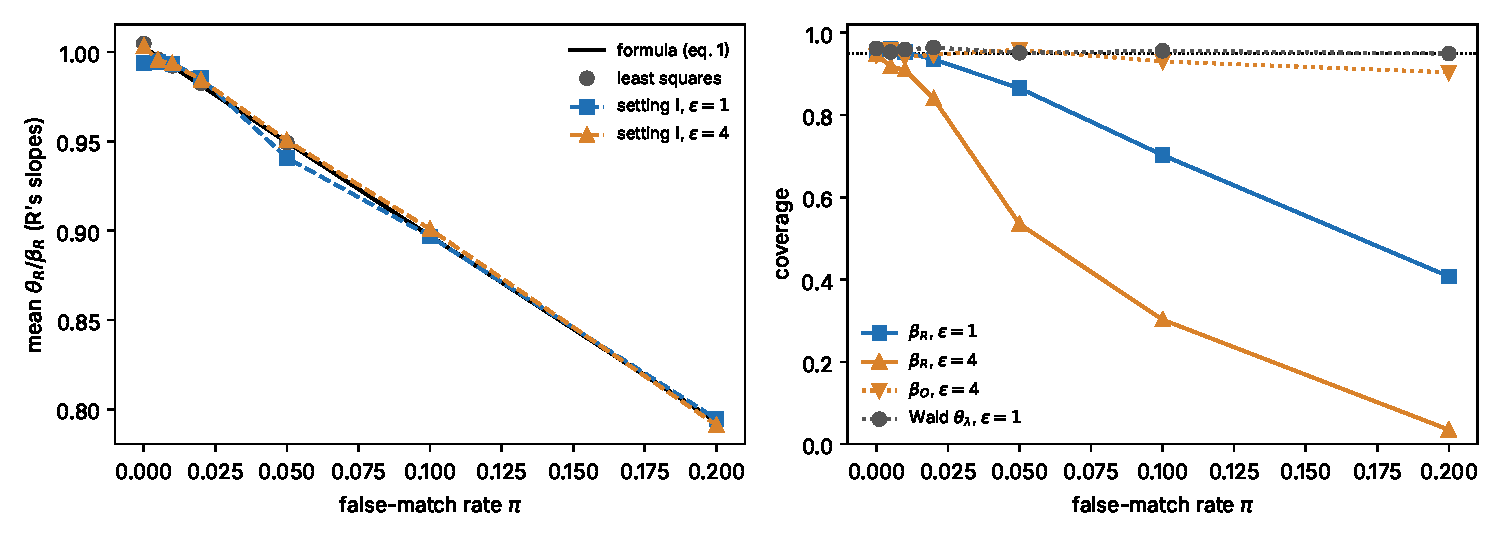
\includegraphics[width=\textwidth]{fig_sweep.pdf}
\caption{Controlled linkage error at $n_0=40{,}000$ true pairs (100 cohorts per point). Left: mean ratio of $\Rp$'s coefficients to the truth, for least squares and for setting~I at $\varepsilon=1,4$, against the contamination formula \eqref{eq:contam}. Right: coverage of the slopes of $\Rp$'s features by the bias-aware interval (nominal 0.95) and of $\btheta_\lambda$ by the Wald interval.}
\label{fig:sweep}
\end{figure}

% ======================================================================
\section{Verdict}
\label{sec:verdict}
\paragraph{Is the idea valid?} \textbf{Partially.} One part is sound and works well: several error-tolerant deterministic keys with an OR rule, linked through today's OPRF-PSI with small protocol changes. The other two parts are not viable in this design: LSH keys, and private Fellegi--Sunter scoring of field agreement.

\paragraph{What works, with numbers.} On a $10^6$-row register with realistic corruption, seven keys and a uniqueness filter link \MKrec\ of the true pairs at precision \MKprec\ (false-match rate \MKfalse). Exact matching on the clean quasi-identifiers links \EXrec\ at \EXprec. Requiring two agreeing keys trades recall for precision (\MKtworec, \MKtwoprec). On FEBRL4's heavier corruption, the keys reach \FBmkrec\ against \FBexrec. At these error rates the effect on the regression is small at $n\approx40{,}000$. $\Rp$'s coefficients shrink by about the false-match rate, which is below the sampling noise of one cohort, and the bias-aware interval kept its coverage (Table~\ref{tab:regression}). With one PSI instance per key type the cost is about $K$ times today's Link phase: about \CostPerSeven\ minutes of $\Op$ time for $K=7$ at $n_R^{\max}=20{,}000$, against \CostBase\,s today. One joint PSI over all keys would cost \CostJointSeven\ minutes at $20{,}000$ queries and \CostJointSevenBig\ hours at $100{,}000$ (modelled).

\paragraph{What does not work.} LSH band keys are low-entropy by design. Behind the uniqueness filter, LSH loses most of its items and links at precision \LSHprec\ and recall \LSHrec\ on the $10^6$ register. That contamination cut $\Rp$'s least-squares coefficients to \LSHratioR\ of their true values, and the bias-aware interval then covered $\Rp$'s slopes in only \LSHcovR\ of releases at $\varepsilon=1$ (\LSHcovRfour\ at $\varepsilon=4$). Without the filter, LSH returns \LSHmultiCand\ candidate positions for 5{,}000 queries on a register of \LSHmultiN\ rows. That is unacceptable leakage, and it needs multi-labels the PSI does not support. Field-level FS scoring through labeled PSI reveals every candidate's agreement vector. Doing it privately needs circuit-PSI with secure scoring and secure 1:1 resolution, which is a different protocol (Remark~13 of the paper and its consequences).

\paragraph{Conditions for validity.}
\begin{enumerate}
\item \emph{Key entropy.} Every key must be close to unique in a register of $\bar n_O$ rows (three or more fields, one of them DOB or postcode). The uniqueness filter turns residual collisions into misses instead of false matches. Precision falls only slowly with register size, from 99.9\% at $10^5$ rows to 99.3\% at $10^6$ and 98.3\% at $3\times10^6$ (Table~\ref{tab:scale}), roughly in step with the share of key values the filter removes. Registers well above $10^6$ rows (all of Canada, $4\times10^7$) need a public scope $\Phi$ that keeps $\bar n_O$ moderate, or keys with more entropy.
\item \emph{Error rates.} The regression tolerates a false-match rate $\pi$ only while $\pi\,|\beta_{R,j}|$ is small next to the interval half-width. In our population at $n=40{,}000$, the bias-aware coverage of $\Rp$'s slopes stays nominal up to $\pi\approx2\%$ at $\varepsilon=1$, where the DP noise dominates. At $\varepsilon=4$ it already drops to about $0.91$ at $\pi=0.5$--$1\%$, then to \SwCovRfourTwo\ at $2\%$, \SwCovRfourFive\ at $5\%$ and \SwCovRfourTen\ at $10\%$. At $\varepsilon=1$ it is \SwCovRoneFive\ at $5\%$ and \SwCovRoneTen\ at $10\%$ (Table~\ref{tab:sweep}). The tolerable $\pi$ shrinks as $n$ and $\varepsilon$ grow. The multikey scheme's $0.7\%$ is at the edge for $\varepsilon=4$. The Wald interval for $\btheta_\lambda$ kept nominal coverage in every cell, but its estimand is the contaminated one. Misses at random cost only sample size, and through it the ridge: at $30\%$ misses ($n\approx28{,}000$, near $n_{\mathrm{off}}=\NoffIone$ at $\varepsilon=1$) the ridge was on in about 80\% of releases. Misses that depend on the outcome bias every coefficient. In our strong MNAR cell (miss probability $\propto e^{-y}$, 30\% on average), $\Rp$'s ratio was \SwMNARratio\ and $\Op$'s \SwMNARratioO. In the MNAR world, exact linkage on the clean quasi-identifiers recovered only \EXrecMNAR\ of the pairs, against \MKrecMNAR\ for the keys, so good recall is itself a defence against selection bias.
\item \emph{Cost.} The budget is $K$ times today's Link phase (OPRF over $K\bar n_O$ inputs, $K$ PSI instances); $K\approx5$--$8$ is affordable at $10^6$ rows.
\item \emph{Variables.} No DP-protected variable, and no function of one, may enter a key.
\end{enumerate}

\paragraph{What must be added to the protocol.}
\begin{enumerate}
\item Public key definitions, a public nickname or normalisation table, and public $K$, agreed in Setup. $\Rp$ pads to exactly $K$ keys per padded record.
\item $K$ PSI instances, one per key type, with $\Op$'s uniqueness filter, and random dummies in place of filtered or missing keys so that sizes stay public.
\item A resolution step at $\Rp$ (FS weights with $u$ from $\Rp$'s own file, then greedy 1:1 with drop-on-tie) in place of the injectivity abort. The final alignment must be injective on $\Op$'s positions (Proposition~\ref{prop:sens}(i)).
\item A restated G4: $\Rp$ learns $\mathcal L_K$, the key-level match function, including agreement patterns, the positions of non-cohort people with a shared key, and cross-key profiles. This must be accepted by $\Op$'s data stewards as part of the disclosure review.
\item Reporting of linkage error. The protocol's intervals should be described as conditional on the linkage. The bias-aware interval for $\bbeta$ does not cover linkage bias, so the published coefficients of $\Rp$'s features should carry the estimated false-match rate as a caveat.
\end{enumerate}

\paragraph{Open problems.} (1) A false-match rate estimate that $\Rp$ can trust without seeing $\Op$'s data, and an interval that remains valid under linkage error. A moment correction exists under the exchangeable model, but it needs $\pi$ and a DP release of $\Op$'s scope means. (2) Hiding the agreement patterns and cross-key joins without giving up $\Rp$'s exact $\bA$. Today this needs circuit-PSI and moves the design to the membership-hiding variant. (3) Robustness to a deviating $\Rp$, which could spend its $K n_R^{\max}$ OPRF budget on low-entropy keys to map the register's frequency structure. (4) Non-exchangeable false matches (households, twins), whose bias depends on the data. (5) Choosing keys and thresholds without access to linked truth, e.g.\ from public reference data or a synthetic generator calibrated to the register.


\begin{thebibliography}{99}\small
\bibitem{rfc9497} A.~Davidson, A.~Faz-Hern\'andez, N.~Sullivan, and C.~A.~Wood, ``Oblivious pseudorandom functions (OPRFs) using prime-order groups,'' RFC~9497, 2023.
\bibitem{jarecki2014round} S.~Jarecki, A.~Kiayias, and H.~Krawczyk, ``Round-optimal password-protected secret sharing and T-PAKE in the password-only model,'' ASIACRYPT 2014.
\bibitem{chen2017fast} H.~Chen, K.~Laine, and P.~Rindal, ``Fast private set intersection from homomorphic encryption,'' ACM CCS 2017.
\bibitem{pinkas2019efficient} B.~Pinkas, T.~Schneider, O.~Tkachenko, and A.~Yanai, ``Efficient circuit-based PSI with linear communication,'' EUROCRYPT 2019.
\bibitem{rindal2021vole} P.~Rindal and P.~Schoppmann, ``VOLE-PSI: fast OPRF and circuit-PSI from vector-OLE,'' EUROCRYPT 2021.
\bibitem{freedman2004efficient} M.~J.~Freedman, K.~Nissim, and B.~Pinkas, ``Efficient private matching and set intersection,'' EUROCRYPT 2004.
\bibitem{chmielewski2008fuzzy} {\L}.~Chmielewski and J.-H.~Hoepman, ``Fuzzy private matching,'' ARES 2008.
\bibitem{indyk2006polylogarithmic} P.~Indyk and D.~Woodruff, ``Polylogarithmic private approximations and efficient matching,'' TCC 2006.
\bibitem{uzun2021fuzzy} E.~Uzun, S.~P.~Chung, V.~Kolesnikov, A.~Boldyreva, and W.~Lee, ``Fuzzy labeled private set intersection with applications to private real-time biometric search,'' USENIX Security 2021.
\bibitem{garimella2022structure} G.~Garimella, M.~Rosulek, and J.~Singh, ``Structure-aware private set intersection, with applications to fuzzy matching,'' CRYPTO 2022.
\bibitem{chakraborti2023distance} A.~Chakraborti, G.~Fanti, and M.~K.~Reiter, ``Distance-aware private set intersection,'' USENIX Security 2023.
\bibitem{vanbaarsen2024fuzzy} A.~van~Baarsen and S.~Pu, ``Fuzzy private set intersection with large hyperballs,'' EUROCRYPT 2024.
\bibitem{broder1997resemblance} A.~Z.~Broder, ``On the resemblance and containment of documents,'' Compression and Complexity of Sequences, 1997.
\bibitem{charikar2002similarity} M.~S.~Charikar, ``Similarity estimation techniques from rounding algorithms,'' STOC 2002.
\bibitem{schnell2009privacy} R.~Schnell, T.~Bachteler, and J.~Reiher, ``Privacy-preserving record linkage using Bloom filters,'' BMC Med.\ Inform.\ Decis.\ Mak.\ 9:41, 2009.
\bibitem{vatsalan2013taxonomy} D.~Vatsalan, P.~Christen, and V.~S.~Verykios, ``A taxonomy of privacy-preserving record linkage techniques,'' Information Systems 38(6), 2013.
\bibitem{christen2020linking} P.~Christen, T.~Ranbaduge, and R.~Schnell, \emph{Linking Sensitive Data}, Springer, 2020.
\bibitem{kuzu2011constraint} M.~Kuzu, M.~Kantarcioglu, E.~Durham, and B.~Malin, ``A constraint satisfaction cryptanalysis of Bloom filters in private record linkage,'' PETS 2011.
\bibitem{niedermeyer2014cryptanalysis} F.~Niedermeyer, S.~Steinmetzer, M.~Kroll, and R.~Schnell, ``Cryptanalysis of basic Bloom filters used for privacy preserving record linkage,'' J.\ Privacy and Confidentiality 6(2), 2014.
\bibitem{christen2018precise} P.~Christen, R.~Schnell, D.~Vatsalan, and T.~Ranbaduge, ``Efficient cryptanalysis of Bloom filters for privacy-preserving record linkage,'' PAKDD 2017 \unverified{venue and title; a TKDE follow-up exists}.
\bibitem{vidanage2019efficient} A.~Vidanage, T.~Ranbaduge, P.~Christen, and R.~Schnell, ``Efficient pattern mining based cryptanalysis for privacy-preserving record linkage,'' ICDE 2019 \unverified{bibliographic details}.
\bibitem{inan2008hybrid} A.~Inan, M.~Kantarcioglu, E.~Bertino, and M.~Scannapieco, ``A hybrid approach to private record linkage,'' ICDE 2008.
\bibitem{he2017composing} X.~He, A.~Machanavajjhala, C.~Flynn, and D.~Srivastava, ``Composing differential privacy and secure computation: a case study on scaling private record linkage,'' ACM CCS 2017.
\bibitem{fellegi1969theory} I.~P.~Fellegi and A.~B.~Sunter, ``A theory for record linkage,'' JASA 64, 1969.
\bibitem{winkler1988using} W.~E.~Winkler, ``Using the EM algorithm for weight computation in the Fellegi--Sunter model of record linkage,'' Proc.\ Section on Survey Research Methods, ASA, 1988.
\bibitem{neter1965effect} J.~Neter, E.~S.~Maynes, and R.~Ramanathan, ``The effect of mismatching on the measurement of response errors,'' JASA 60, 1965.
\bibitem{scheuren1993regression} F.~Scheuren and W.~E.~Winkler, ``Regression analysis of data files that are computer matched,'' Survey Methodology 19, 1993.
\bibitem{lahiri2005regression} P.~Lahiri and M.~D.~Larsen, ``Regression analysis with linked data,'' JASA 100, 2005.
\bibitem{chambers2009regression} R.~Chambers, ``Regression analysis of probability-linked data,'' Official Statistics Research Series, Statistics New Zealand, 2009 \unverified{series and year}.
\bibitem{lin2024differentially} S.~Lin, E.~Paquette, and E.~D.~Kolaczyk, ``Differentially private linear regression with linked data,'' Harvard Data Science Review 6(3), 2024.
\bibitem{christen2008febrl} P.~Christen, ``Febrl: a freely available record linkage system with a graphical user interface,'' HDKM 2008.
\end{thebibliography}
\end{document}
